\chapter{Técnicas de laboratório III: a prática da pesquisa}\label{ch:b3:lab-techniques-3}

Um frasco de solução de butil-lítio pega fogo se uma gota encontra o ar; uma
\omterm{def:b3:lab-techniques-3:schlenk}{caixa de luvas} mantém o oxigênio e a água abaixo de algumas partes por milhão para que esses
compostos possam ser pesados como sal de cozinha. A química de pesquisa muitas vezes começa
mantendo a atmosfera do lado de fora e termina com uma afirmação que outros precisam poder
verificar: um composto novo, com estrutura e pureza provadas por vários métodos
independentes, e seus dados registrados e publicados para que o trabalho possa ser repetido. Este
último capítulo reúne a prática da pesquisa: manipular substâncias sensíveis ao ar,
caracterizar um composto novo, julgar estatisticamente um resultado,
manter um \omterm{def:b3:lab-techniques-3:notebook}{caderno de laboratório} e ler a literatura, e avaliar os riscos de um
procedimento que ninguém jamais executou.

\begin{recall}
O volume do 1.º ano tratou dos perigos, dos riscos, dos pictogramas, das frases H e P, das fichas de dados de
segurança e da incerteza de medida, com suas avaliações dos tipos A e B; o
volume do 2.º ano, das atmosferas inertes, do isolamento, dos agentes secantes, da cromatografia flash,
da espectrometria de massa (HRMS, massa monoisotópica), da RMN de $^{13}$C, dos intervalos de confiança,
do coeficiente de Student, da calibração, da precisão, da veracidade, do viés, da repetibilidade,
da validação de métodos, da elevação adiabática de temperatura e da perda de controle térmico.
O \cref{ch:b3:advanced-nmr}, o \cref{ch:b3:x-ray-diffraction} e o
\cref{ch:b3:electrode-kinetics} forneceram os métodos estruturais e
eletroquímicos.
\end{recall}

\begin{omfigure}
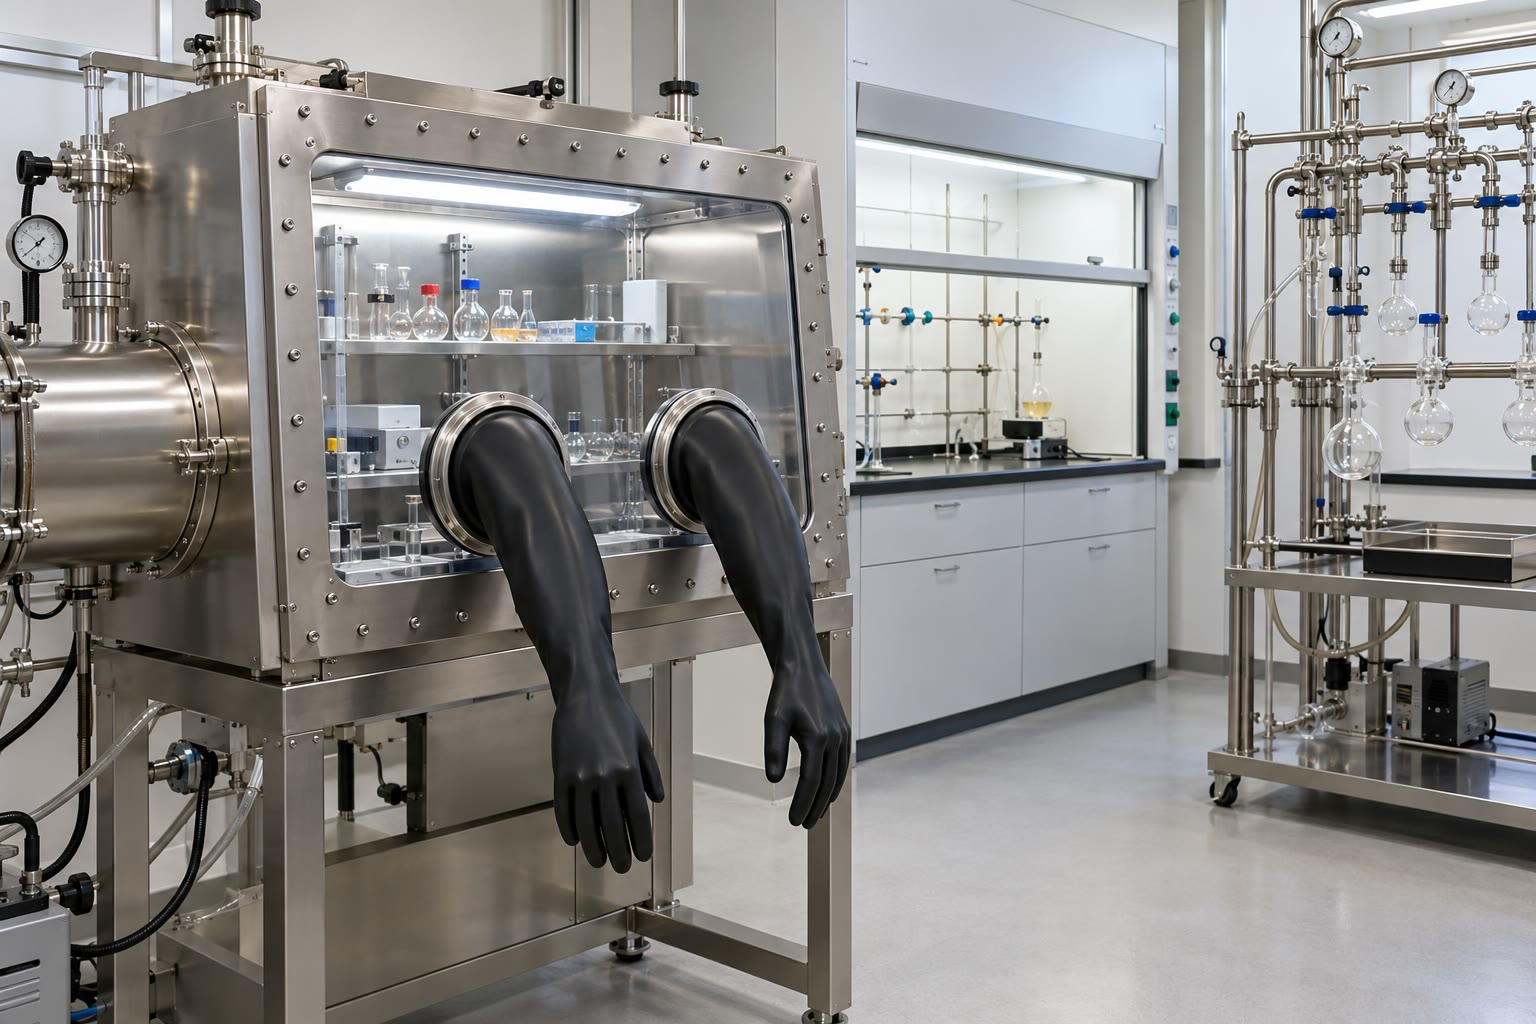
\includegraphics[width=0.58\linewidth]{images/book4/ai/b3-33-glovebox.jpg}

{\small Um laboratório de pesquisa com uma \omterm{def:b3:lab-techniques-3:schlenk}{caixa de luvas}: a caixa de aço inoxidável, cheia
de nitrogênio ou de argônio secos, é acessada pelas luvas; o cilindro à
esquerda é a antecâmara para introduzir e retirar objetos.}
\end{omfigure}

\section{Trabalhar sem ar}

\begin{definition}[Compostos sensíveis ao ar]\label{def:b3:lab-techniques-3:air-sensitive}
Um \emph{composto sensível ao ar}\index{composto sensivel ao ar@composto sensível ao ar} reage com o
dioxigênio ou com a água do ar, decompondo-se ou perdendo sua atividade. Uma
\emph{substância pirofórica}\index{substancia piroforica@substância pirofórica} se inflama espontaneamente
ao ar.
\end{definition}

\begin{definition}[Linha de Schlenk e caixa de luvas]\label{def:b3:lab-techniques-3:schlenk}
Uma \emph{linha de Schlenk}\index{linha de Schlenk} é um coletor duplo de vidro, com um tubo
ligado a uma bomba de vácuo por meio de uma armadilha fria e o outro a uma fonte de gás inerte
seco que escapa por um borbulhador de óleo, com torneiras que ligam cada saída a
um ou a outro. Um \emph{frasco de Schlenk}\index{frasco de Schlenk} tem um braço lateral com torneira
para ligação à linha. Uma \emph{caixa de luvas}\index{caixa de luvas} é uma caixa fechada
cheia de gás inerte, purificado continuamente, na qual se trabalha por meio de
luvas.
\end{definition}

\begin{omfigure}
\begin{tikzpicture}[font=\scriptsize, >=Stealth]
  % manifolds
  \draw[om glass, line width=1.1pt] (0,3.0) -- (8.0,3.0);
  \draw[om glass, line width=1.1pt] (0,2.5) -- (8.0,2.5);
  \node[anchor=east] at (-1.0,3.0) {gás inerte};
  \node[anchor=east] at (0,2.5) {vácuo};
  % taps
  \foreach \x in {2.0,4.0,6.0} {
    \draw[om glass] (\x,3.0) -- (\x,2.5);
    \draw[fill=white] (\x,2.75) circle (0.12);
    \draw (\x-0.1,2.75) -- (\x+0.1,2.75);
    \draw[om glass] (\x,2.5) -- (\x,2.0);
  }
  % flask on the middle tap
  \draw[thick, black!60] (4.0,2.0) -- (4.0,1.6) -- (4.6,1.6);
  \pic[scale=0.5, transform shape] at (5.0,-0.2) {rbflask={0.3}{omDef!20}};
  \draw[om glass] (4.6,1.6) -- (4.9,1.25);
  \node[anchor=west] at (5.4,0.4) {frasco de Schlenk};
  % bubbler at the gas end
  \pic[scale=0.55, transform shape] at (8.9,1.5) {bubbler};
  \draw[om glass] (8.0,3.0) -- (8.6,3.0) -- (8.6,2.9);
  \node[anchor=west] at (9.4,2.2) {borbulhador de óleo};
  % trap and pump at the vacuum end
  \draw[om glass] (0.4,2.5) -- (0.4,1.6);
  \draw[om glass, fill=omDef!8] (0.15,1.6) rectangle (0.65,0.4);
  \fill[omDef!25] (0.0,0.2) rectangle (0.8,1.2);
  \node[anchor=north] at (0.4,0.2) {armadilha fria};
  \draw[om glass] (0.65,0.9) -- (1.6,0.9);
  \draw[fill=black!15] (1.6,0.6) rectangle (2.6,1.2);
  \node at (2.1,0.9) {bomba};
  \draw[->, thick] (-0.9,3.0) -- (0,3.0);
\end{tikzpicture}

{\small Uma \omterm{def:b3:lab-techniques-3:schlenk}{linha de Schlenk}, esquemática: um coletor de gás e um coletor de vácuo ligados por
torneiras; cada torneira liga seu frasco ao vácuo ou ao gás inerte. O vapor de solvente
bombeado se condensa na armadilha fria antes de chegar à bomba; o gás sai
por um borbulhador de óleo, que impede o refluxo do ar.}
\end{omfigure}

\begin{proposition}[Ciclos de evacuação e reenchimento]\label{prop:b3:lab-techniques-3:purge-cycles}
Se um frasco cheio de ar à pressão $p_0$ é evacuado até $p_{\min}$ e reenchido com
gás inerte puro, $n$ vezes, a fração do ar original que resta é $(p_{\min}/p_0)^n$.
\end{proposition}

\begin{proof}
A evacuação até $p_{\min}$ deixa uma fração $p_{\min}/p_0$ do gás, de mesma composição; o
reenchimento com gás inerte puro restabelece $p_0$ sem acrescentar ar. Cada ciclo multiplica a
fração de ar por $p_{\min}/p_0$; após $n$ ciclos, $(p_{\min}/p_0)^n$.
\end{proof}

Três ciclos até \qty{0.1}{mbar} deixam, no papel, $10^{-12}$ do ar; na prática, os vazamentos, o gás
adsorvido no vidro e a liberação de gases pela graxa e pelos septos fixam o limite, e é
por isso que a vidraria é seca em estufa e montada quente.

\begin{definition}[Transferência por cânula]\label{def:b3:lab-techniques-3:cannula}
Uma \emph{transferência por cânula}\index{transferencia por canula@transferência por cânula} desloca um líquido sensível ao ar
de um recipiente fechado para outro por uma longa agulha de duas pontas, impulsionado
por uma pequena sobrepressão de gás inerte no primeiro recipiente.
\end{definition}

\begin{omfigure}
\begin{tikzpicture}[font=\scriptsize, >=Stealth]
  \pic at (0,0) {rbflask={0.35}{omThm!25}};
  \pic at (4.2,0) {rbflask={0.1}{omDef!15}};
  \pic at (0,3.0) {septum};
  \pic at (4.2,3.0) {septum};
  \draw[black!70, line width=0.9pt] (0.05,0.25) -- (0.05,3.5) to[out=90, in=90] (4.15,3.5) -- (4.15,1.6);
  \draw[->, thick, omThm] (1.3,3.95) -- (2.9,3.95) node[midway, above] {líquido};
  \draw[->, thick] (-1.3,3.4) -- (-0.15,3.2) node[pos=0, left] {entrada de gás inerte (leve sobrepressão)};
  \draw[->, thick] (4.35,3.2) -- (5.4,3.6) node[right] {saída para o borbulhador};
  \node[anchor=north] at (0,-0.1) {origem};
  \node[anchor=north] at (4.2,-0.1) {destino};
\end{tikzpicture}

{\small Uma \omterm{def:b3:lab-techniques-3:cannula}{transferência por cânula}: a ponta inferior da cânula mergulha no líquido do
frasco de origem; o gás inerte introduzido na origem empurra o líquido pela
cânula até o frasco de destino, que tem uma saída por uma agulha para o borbulhador.}
\end{omfigure}

\begin{method}[Uma transferência por cânula]\label{met:b3:lab-techniques-3:cannula}
\begin{enumerate}
  \item Coloque os dois frascos, fechados com septos, sob gás inerte na \omterm{def:b3:lab-techniques-3:schlenk}{linha de Schlenk}.
  \item Purgue a cânula com gás: insira uma extremidade na origem, acima do líquido,
        até que o gás saia pela outra extremidade, depois insira essa extremidade no destino.
  \item Dê saída ao destino com uma agulha; empurre a extremidade da cânula na origem para baixo da
        superfície do líquido: a sobrepressão impulsiona o líquido.
  \item Para parar, levante a ponta acima do líquido; retire primeiro a cânula do destino
        e lave-a imediatamente com um solvente seco, depois com água, na capela.
\end{enumerate}
\end{method}

\begin{definition}[Desgaseificação por congelamento--bombeamento--descongelamento]\label{def:b3:lab-techniques-3:degassing}
A \emph{desgaseificação por congelamento--bombeamento--descongelamento}\index{desgaseificacao por congelamento--bombeamento--descongelamento@desgaseificação por congelamento--bombeamento--descongelamento} remove
os gases dissolvidos de um líquido congelando-o em nitrogênio líquido, evacuando o
espaço acima dele, fechando a torneira e deixando-o descongelar, de modo que o gás dissolvido escape
para o vácuo; o ciclo é repetido três vezes.
\end{definition}

Os solventes secos vêm hoje de colunas de alumina ativada sob gás inerte,
e não de destiladores sobre sódio. As soluções de organolítio perdem concentração com o
tempo e são tituladas antes do uso, por exemplo contra uma quantidade pesada de
ácido difenilacético em THF seco: o primeiro equivalente desprotona o ácido, e a
primeira gota em excesso dá o diânion amarelo.

\begin{proposition}[Título de um organolítio]\label{prop:b3:lab-techniques-3:titre}
Se uma massa $m$ de ácido difenilacético (massa molar $M$) exige um volume $V$ de uma
solução de organolítio para atingir a mudança de cor, a concentração é $c = m/(MV)$.
\end{proposition}

\begin{proof}
Até o ponto final, cada organolítio retira um próton do ácido; a
cor aparece quando o ácido se esgota. As quantidades são iguais: $cV = m/M$.
\end{proof}

\begin{inthelab}[A antecâmara da caixa de luvas]
Os objetos entram em uma \omterm{def:b3:lab-techniques-3:schlenk}{caixa de luvas} por sua antecâmara: são colocados dentro dela, a
porta externa é fechada, e a câmara é evacuada e reenchida com o gás da caixa
três vezes, com uma longa evacuação final para os objetos porosos, que retêm ar;
só então a porta interna é aberta de dentro da caixa com as luvas. Os solventes
e os recipientes abertos de líquidos voláteis nunca são bombeados na antecâmara, e
nada que possa envenenar o purificador (tióis, solventes halogenados) é aberto
dentro dela sem autorização.
\end{inthelab}

\begin{omfigure}
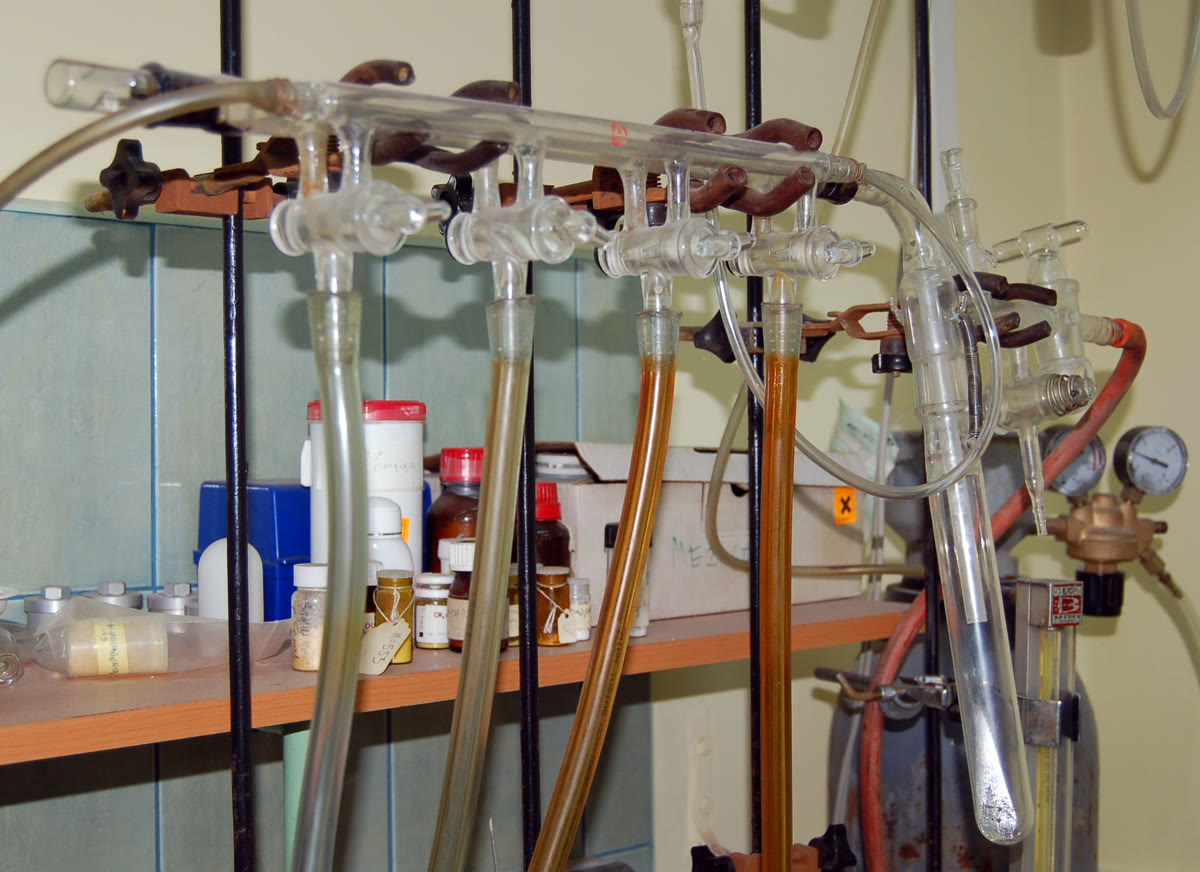
\includegraphics[width=0.46\linewidth]{images/book4/schlenk-line.jpg}

{\small Uma \omterm{def:b3:lab-techniques-3:schlenk}{linha de Schlenk} em uso: o coletor de vidro com suas torneiras, os tubos que vão aos
frascos e o regulador de gás. Fotografia: Polimerek, CC BY-SA 3.0.}
\end{omfigure}

\section{Caracterizar um composto novo}

\begin{method}[Caracterizar um composto novo]\label{met:b3:lab-techniques-3:characterise}
\begin{enumerate}
  \item Pureza: uma única mancha em CCD em dois eluentes, um único pico em HPLC ou em CG, um ponto de fusão
        nítido; \omterm{def:b3:lab-techniques-3:qnmr}{RMN quantitativa} se for necessária uma pureza em massa.
  \item Fórmula: HRMS a poucos ppm da massa calculada, e o perfil
        isotópico; ou \omterm{def:b3:lab-techniques-3:elemental}{análise elementar}.
  \item Estrutura: RMN de $^1$H e de $^{13}$C com experimentos 2D para as conexões
        (\cref{ch:b3:advanced-nmr}), IV para os grupos funcionais; uma estrutura de
        raios X em monocristal quando os cristais crescem (\cref{ch:b3:x-ray-diffraction}).
  \item Estereoquímica: NOE, constantes de acoplamento, poder rotatório, ee por
        cromatografia quiral.
  \item Relate cada dado com suas condições, e os espectros no \omterm{def:b3:lab-techniques-3:literature}{material
        suplementar}.
\end{enumerate}
\end{method}

\begin{omfigure}
\begin{tikzpicture}[font=\scriptsize, >=Stealth,
  box/.style={draw, rounded corners, align=center, fill=omDef!8, inner sep=3pt, minimum height=8mm}]
  \node[box] (a) at (0,0) {composto novo\\ isolado};
  \node[box] (b) at (2.85,0) {puro?\\ CCD, HPLC,\\ p.f.};
  \node[box] (c) at (5.85,0) {fórmula\\ HRMS, CHN};
  \node[box] (d) at (8.75,0) {estrutura\\ RMN (1D, 2D), IV};
  \node[box] (e) at (8.75,-1.6) {raios X (se houver\\ cristais),\\ estereoquímica};
  \node[box, fill=omMeth!12] (f) at (5.85,-1.6) {coerente?\\ relatar com os\\ dados brutos};
  \node[box, fill=omThm!10] (g) at (2.85,-1.6) {purificar de novo\\ (cromatografia,\\ cristalização)};
  \draw[->, thick] (a) -- (b); \draw[->, thick] (b) -- node[above, inner sep=1pt] {sim} (c);
  \draw[->, thick] (c) -- (d); \draw[->, thick] (d) -- (e); \draw[->, thick] (e) -- (f);
  \draw[->, thick] (b) -- node[left] {não} (g); \draw[->, thick] (g.north west) to[bend left=30] (a.south);
\end{tikzpicture}

{\small O fluxo de caracterização de um composto novo: primeiro a pureza, depois a
fórmula, depois a estrutura; toda afirmação se apoia em pelo menos dois métodos
independentes, e os \omterm{def:b3:lab-techniques-3:notebook}{dados brutos} acompanham o relatório.}
\end{omfigure}

\begin{definition}[Análise elementar]\label{def:b3:lab-techniques-3:elemental}
A \emph{análise elementar}\index{analise elementar@análise elementar} (análise por combustão)
determina as porcentagens em massa de carbono, hidrogênio, nitrogênio e enxofre de uma
amostra queimando-a em oxigênio e medindo o dióxido de carbono, a água, o
dinitrogênio e o dióxido de enxofre formados.
\end{definition}

\begin{proposition}[Porcentagens em massa a partir de uma fórmula]\label{prop:b3:lab-techniques-3:mass-fractions}
Para uma fórmula $\mathrm{C}_a\mathrm{H}_b\mathrm{N}_c\dots$ de massa molar $M$, a porcentagem em massa de carbono é $100\,aA_r(\mathrm C)/M$, e do mesmo modo
para os outros elementos.
\end{proposition}

\begin{proof}
Um mol de composto, de massa $M$, contém $a$ mols de átomos de carbono, de massa $aA_r(\mathrm C)$;
a razão, vezes 100, é a porcentagem em massa.
\end{proof}

% ledger: ea:tolerance, hrms:tolerance
A maioria das revistas de química exige valores encontrados de C, H e N a menos de 0.4 ponto
percentual dos calculados, ou uma medida de HRMS a poucos ppm (5 ppm
para algumas), como prova da composição. Um grande estudo interlaboratorial verificou que
mesmo amostras puras deixam de atender ao critério de 0.4 com surpreendente frequência, um lembrete de que um
critério não é uma lei da natureza.

\begin{proposition}[Erro em HRMS]\label{prop:b3:lab-techniques-3:ppm-error}
O erro de uma massa medida $m_{\mathrm{meas}}$ em relação à massa calculada $m_{\mathrm{calc}}$ é
$10^6(m_{\mathrm{meas}} - m_{\mathrm{calc}})/m_{\mathrm{calc}}$ ppm; para um íon, $m_{\mathrm{calc}}$ é calculada a partir das massas monoisotópicas menos (ou mais) a
massa dos elétrons retirados (ou acrescentados).
\end{proposition}

\begin{proof}[Por definição]
O erro em ppm é a diferença relativa expressa em partes por milhão; a
massa do íon difere da da fórmula neutra pelos elétrons, \qty{5.486e-4}{u} cada um, alguns
ppm para massas de algumas centenas.
\end{proof}

\begin{definition}[RMN quantitativa]\label{def:b3:lab-techniques-3:qnmr}
A \emph{RMN quantitativa}\index{RMN quantitativa} (qNMR) determina quantidades ou
purezas a partir das integrais dos sinais, que são proporcionais ao número de núcleos
quando o espectro é registrado com relaxação completa entre os pulsos, em relação a um
padrão interno de pureza conhecida pesado junto com a amostra.
\end{definition}

\begin{proposition}[Pureza por qNMR]\label{prop:b3:lab-techniques-3:qnmr}
Para uma amostra de massa $m_x$ pesada com um padrão de massa $m_s$ e pureza $P_s$, com sinais
de integrais $I_x$ e $I_s$ provenientes de $N_x$ e $N_s$ prótons,
\[
  P_x = \frac{I_x}{I_s}\,\frac{N_s}{N_x}\,\frac{M_x}{M_s}\,\frac{m_s}{m_x}\,P_s.
\]
\end{proposition}

\begin{proof}
As integrais são proporcionais aos números de prótons: $I_x/I_s = (N_xn_x)/(N_sn_s)$. Com
$n_x = P_xm_x/M_x$ e $n_s = P_sm_s/M_s$, resolver para $P_x$ dá a fórmula.
\end{proof}

\begin{omfigure}
\begin{tikzpicture}
\begin{axis}[width=0.8\linewidth, height=5.0cm, x dir=reverse, xmin=3.0, xmax=7.0, ymin=-0.05, ymax=1.15, clip=false,
  axis x line=bottom, axis y line=none, xlabel={$\delta$ / ppm}, tick label style={font=\scriptsize}, label style={font=\small}]
\addplot[color=omDef, thick] table[x=ppm, y=y] {figdata/out/bachelor-3-qnmr.dat};
\node[font=\scriptsize, anchor=south] at (axis cs:6.09,0.33) {padrão, ArH (3 H)};
\node[font=\scriptsize, anchor=east] at (axis cs:4.20,0.98) {ferroceno (10 H)};
\node[font=\scriptsize, anchor=west, align=left] at (axis cs:3.72,0.70) {padrão,\\ $\ce{OCH3}$ (9 H)};
\end{axis}
\end{tikzpicture}

{\small Espectro de prótons sintético de uma amostra de ferroceno pesada com
1,3,5-trimetoxibenzeno como padrão interno (modelo: 20.0 mg de amostra de 98.0\,\% de
pureza, 15.0 mg de padrão). As integrais são proporcionais ao número de
prótons vezes a quantidade de cada composto; a razão entre o singleto do ferroceno e
o singleto aromático do padrão dá a pureza.}
\end{omfigure}

\section{Estatística de um resultado de pesquisa}

\begin{definition}[Testes de significância]\label{def:b3:lab-techniques-3:tests}
Um \emph{teste de significância}\index{teste de significancia@teste de significância} decide se os dados são
compatíveis com uma \emph{hipótese nula}\index{hipotese nula@hipótese nula}, em geral a de que
não há diferença ou efeito, a um nível escolhido de risco de rejeitá-la
erroneamente (muitas vezes 5\,\%).
\end{definition}

\begin{theorem}[Teste $t$ para duas amostras]\label{thm:b3:lab-techniques-3:t-test}
Para dois conjuntos de $n_1$ e $n_2$ medidas independentes provenientes de distribuições
normais de mesmo desvio-padrão, com médias $\bar x_1$, $\bar x_2$ e desvio-padrão combinado
$s_p$, a estatística $t = (\bar x_1 - \bar x_2)/(s_p\sqrt{1/n_1 + 1/n_2})$ segue a lei de Student com
$n_1 + n_2 - 2$ graus de liberdade quando as duas médias verdadeiras são iguais. \admitted
\end{theorem}

\begin{proposition}[Teste $F$]\label{prop:b3:lab-techniques-3:f-test}
Sob as mesmas hipóteses, a razão $F = s_1^2/s_2^2$ de duas variâncias amostrais segue
a lei de Fisher com $(n_1 - 1, n_2 - 1)$ graus de liberdade quando as variâncias verdadeiras são iguais.
\admitted
\end{proposition}

\begin{method}[Um novo rendimento é melhor?]\label{met:b3:lab-techniques-3:compare-means}
\begin{enumerate}
  \item Repita os dois procedimentos várias vezes nas mesmas condições; registre
        todos os resultados.
  \item Compare primeiro as dispersões (teste $F$); se forem semelhantes, combine-as:
        $s_p^2 = [(n_1 - 1)s_1^2 + (n_2 - 1)s_2^2]/(n_1 + n_2 - 2)$.
  \item Calcule $t$ e compare $|t|$ com o coeficiente de Student para $n_1 + n_2 - 2$ graus de
        liberdade ao nível escolhido.
  \item Maior: a diferença é significativa. Menor: os dados não a mostram,
        o que não prova que ela não exista.
\end{enumerate}
\end{method}

Um valor suspeito nunca é eliminado por ser incômodo. Os testes de valores aberrantes
o sinalizam, mas a decisão se apoia no caderno: uma causa registrada (um erro de
pesagem, um frasco contaminado) justifica rejeitá-lo; sem ela, ele é mantido,
ou o experimento é repetido.

\section{O caderno, os dados de pesquisa e a literatura}

\begin{definition}[Caderno e dados brutos]\label{def:b3:lab-techniques-3:notebook}
O \emph{caderno de laboratório}\index{caderno de laboratorio@caderno de laboratório} é o registro datado,
contínuo e inalterado dos experimentos realizados, tal como foram realizados. Os \emph{dados
brutos}\index{dados brutos} são os registros originais das medidas (arquivos dos
instrumentos, tíquetes de pesagem, espectros) antes de qualquer tratamento.
\end{definition}

\begin{method}[Redigir uma entrada no caderno]\label{met:b3:lab-techniques-3:notebook}
\begin{enumerate}
  \item Data, título, objetivo e uma referência ao experimento relacionado anterior.
  \item O esquema da reação com as quantidades (massas, volumes, mols, equivalentes),
        as origens e os lotes dos reagentes, e a \omterm{def:b3:lab-techniques-3:assessment}{avaliação de riscos}.
  \item O que foi feito e observado, em ordem e no momento, inclusive o que deu
        errado; nunca apague, risque de modo que o original permaneça legível.
  \item Resultados: rendimentos, os nomes dos arquivos de \omterm{def:b3:lab-techniques-3:notebook}{dados brutos} e uma conclusão; assine.
\end{enumerate}
\end{method}

\begin{definition}[Dados FAIR]\label{def:b3:lab-techniques-3:fair}
% ledger: fair:year
Os \emph{dados FAIR}\index{dados FAIR} são dados de pesquisa localizáveis,
acessíveis, interoperáveis e reutilizáveis (as iniciais da sigla em inglês): descritos com metadados ricos e um
identificador persistente, recuperáveis por protocolos padronizados, em formatos abertos, com
uma licença e uma procedência claras.
\end{definition}

\begin{definition}[Integridade científica]\label{def:b3:lab-techniques-3:integrity}
A \emph{integridade científica}\index{integridade cientifica@integridade científica} é a condução e a divulgação
honestas e transparentes da pesquisa. Suas violações mais graves são a
\emph{fabricação}\index{fabricacao@fabricação} (inventar dados), a \emph{falsificação}\index{falsificacao@falsificação}
(alterar dados, imagens ou procedimentos) e o \emph{plágio}\index{plagio@plágio}
(apresentar como próprio o trabalho de outros).
\end{definition}

\begin{definition}[A literatura]\label{def:b3:lab-techniques-3:literature}
A \emph{literatura primária}\index{literatura primaria@literatura primária} relata pesquisas
originais (artigos, patentes, teses); a \emph{literatura
secundária}\index{literatura secundaria@literatura secundária} as revisa e organiza (artigos de revisão,
manuais, bases de dados), e os livros didáticos formam uma camada terciária. A \emph{revisão
por pares}\index{revisao por pares@revisão por pares} é a avaliação de um manuscrito por especialistas independentes
antes da publicação. O \emph{material suplementar}\index{material suplementar}
de um artigo contém os detalhes experimentais e os dados necessários para
repetir e verificar o trabalho.
\end{definition}

\begin{method}[Ler um procedimento publicado]\label{met:b3:lab-techniques-3:read-paper}
\begin{enumerate}
  \item Leia a parte experimental e o \omterm{def:b3:lab-techniques-3:literature}{material suplementar}, não apenas o
        resumo e o esquema.
  \item Verifique a escala, as concentrações, as temperaturas, os tempos e o isolamento; anote
        o que falta.
  \item Verifique a caracterização dos produtos segundo o método acima.
  \item Procure artigos posteriores que usaram ou corrigiram o procedimento; execute-o primeiro em
        pequena escala.
\end{enumerate}
\end{method}

As bases de dados de estruturas e de reações indexam a \omterm{def:b3:lab-techniques-3:literature}{literatura primária} por composto e
por transformação, e são consultadas desenhando uma estrutura ou uma reação,
e não por palavras.

\section{Avaliação de riscos de um novo procedimento}

\begin{definition}[Avaliação de riscos]\label{def:b3:lab-techniques-3:assessment}
Uma \emph{avaliação de riscos}\index{avaliacao de riscos@avaliação de riscos} de um procedimento identifica seus
perigos, estima a probabilidade e a gravidade do dano nas condições previstas
e fixa as medidas de controle que reduzem o risco a um nível aceitável. A
\emph{hierarquia de controles}\index{hierarquia de controles} as classifica da mais à
menos eficaz: eliminação, substituição, controles de engenharia,
controles administrativos, equipamentos de proteção individual.
\end{definition}

\begin{omfigure}
\begin{tikzpicture}[font=\scriptsize]
  \foreach \i/\lab/\col in {0/eliminação: remover o perigo/omMeth!40, 1/substituição: um reagente menos perigoso/omMeth!28, 2/engenharia: capela{,} caixa de luvas{,} anteparos/omDef!22, 3/administrativos: procedimentos{,} treinamento/omProp!22, 4/equipamentos de proteção individual/omThm!22} {
    \pgfmathsetmacro\w{5.4-0.95*\i}
    \fill[\col] ({-\w/2},{-0.75*\i}) -- ({\w/2},{-0.75*\i}) -- ({\w/2-0.475},{-0.75*\i-0.7}) -- ({-\w/2+0.475},{-0.75*\i-0.7}) -- cycle;
    \node[anchor=west] at (3.0,{-0.75*\i-0.35}) {\lab};
    \draw[black!30] ({\w/2-0.2},{-0.75*\i-0.35}) -- (2.95,{-0.75*\i-0.35});
  }
  \node[anchor=east, align=right] at (-2.9,-0.35) {mais\\ eficaz};
  \node[anchor=east, align=right] at (-2.9,-3.35) {menos\\ eficaz};
  \draw[->, black!50] (-3.3,-0.85) -- (-3.3,-2.85);
\end{tikzpicture}

{\small A \omterm{def:b3:lab-techniques-3:assessment}{hierarquia de controles}, como uma pirâmide invertida: eliminar ou substituir
o perigo protege a todos, sempre; o equipamento de proteção só protege quem
o usa, e apenas quando está em uso e intacto.}
\end{omfigure}

\begin{definition}[Formadores de peróxidos]\label{def:b3:lab-techniques-3:peroxide}
Um \emph{formador de peróxidos}\index{formador de peroxidos@formador de peróxidos} é um composto, como o éter
dietílico, o tetra-hidrofurano ou o 1,4-dioxano, que forma lentamente peróxidos explosivos
com o ar durante o armazenamento, sobretudo depois de aberto e na presença de luz.
\end{definition}

\begin{method}[Avaliar os riscos de um novo procedimento]\label{met:b3:lab-techniques-3:risk-assessment}
\begin{enumerate}
  \item Liste todas as substâncias (reagentes, solventes, produtos, subprodutos, gases
        liberados) com seus perigos segundo a ficha de dados de segurança.
  \item Liste as operações e suas condições (aquecimento, pressão, escala,
        neutralização final, resíduos); estime o calor liberado e a elevação adiabática de temperatura
        antes de aumentar a escala.
  \item Para cada perigo, escolha as medidas descendo a hierarquia; planeje a resposta
        de emergência (derramamento, incêndio, exposição) e o destino dos resíduos.
  \item Registre-a por escrito, faça-a verificar e revise-a após a primeira execução.
\end{enumerate}
\end{method}

\begin{safety}{\ghs[0.62cm]{GHS02}\ghs[0.62cm]{GHS05}\ghs[0.62cm]{GHS07}\ghs[0.62cm]{GHS08}}
% ledger: ghs4:BuLi, ghs4:Et2O, ghs4:THF
Soluções de butil-lítio: pirofóricas, reagem violentamente com a água liberando
gás inflamável, provocam queimaduras graves; manipuladas apenas sob gás inerte, com um balde de
areia seca à mão e nenhuma água por perto. O hidreto de sódio também libera
hidrogênio com a água e a umidade, e é usado como dispersão em óleo. O éter
dietílico e o THF são \omterm{def:b3:lab-techniques-3:peroxide}{formadores de peróxidos} altamente inflamáveis: datados na abertura, testados para
peróxidos antes de uma destilação ou evaporação, e descartados conforme o cronograma.
\end{safety}

\begin{history}[A vidraria de Schlenk]
Wilhelm Schlenk, estudando os compostos organoalcalinos e os radicais na década de 1910,
projetou os frascos e as técnicas que lhe permitiram manipulá-los sem ar; a
linha e o frasco ainda levam seu nome. As primeiras \omterm{def:b3:lab-techniques-3:schlenk}{caixas de luvas} foram construídas na
década de 1940 para os materiais radioativos e logo adotadas pelos químicos que trabalhavam com
\omterm{def:b3:lab-techniques-3:air-sensitive}{compostos sensíveis ao ar}.
\end{history}

\section{Exercícios}

\begin{exercise}[$\star$]\label{exo:b3:lab-techniques-3:1}
Um frasco é evacuado até \qty{0.50}{mbar} e reenchido até \qty{1013}{mbar} com argônio três vezes. Que fração do
ar original resta, em teoria? O que limita realmente o resultado?
\end{exercise}

\begin{exercise}[$\star$]\label{exo:b3:lab-techniques-3:2}
Uma solução de butil-lítio tem título de \qty{1.48}{mol/L}. Que volume deve ser transferido para fornecer
\qty{20.0}{mmol}?
\end{exercise}

\begin{exercise}[$\star$]\label{exo:b3:lab-techniques-3:3}
% ledger: mass:C12, mass:H1, mass:Fe56, const4:me.u, hrms:tolerance
Calcule a massa exata do cátion radical do ferroceno $\ce{C10H10Fe+}$ a partir das massas monoisotópicas
($^{12}$C exatamente 12, $^1$H 1.00782503, $^{56}$Fe 55.93493633, elétron \qty{5.486e-4}{u}), e o erro de uma medida de
186.0129 em ppm.
\end{exercise}

\begin{exercise}[$\star$]\label{exo:b3:lab-techniques-3:4}
Classifique como \omterm{def:b3:lab-techniques-3:literature}{literatura primária}, secundária ou terciária: um artigo de revisão, um
artigo de revista que relata uma nova síntese, uma patente, um manual de constantes
físicas, uma tese, um livro didático.
\end{exercise}

\begin{exercise}[$\star\star$]\label{exo:b3:lab-techniques-3:5}
% ledger: ea:tolerance
Calcule as porcentagens em massa de C, H e N da cafeína, $\ce{C8H10N4O2}$, e decida se os valores
encontrados C 49.31, H 5.22, N 28.71\,\% atendem ao critério usual de 0.4 ponto.
\end{exercise}

\begin{exercise}[$\star\star$]\label{exo:b3:lab-techniques-3:6}
Uma amostra de \qty{170.0}{mg} de ácido difenilacético ($\ce{C14H12O2}$) exige \qty{0.54}{mL} de uma solução de butil-lítio para atingir
o ponto final amarelo. Calcule o título.
\end{exercise}

\begin{exercise}[$\star\star$]\label{exo:b3:lab-techniques-3:7}
Um procedimento antigo deu rendimentos de 72, 75, 71, 74 e 73\,\%; um modificado, 76, 78, 75, 77 e
79\,\%. Com o coeficiente de Student 2.31 para 8 graus de liberdade a 95\,\% (dados do exercício),
a melhoria é significativa?
\end{exercise}

\begin{exercise}[$\star\star$]\label{exo:b3:lab-techniques-3:8}
Dois métodos dão seis resultados cada um, com desvios-padrão de 0.80 e 0.30 (mesmas
unidades). Com um $F$ crítico de 5.05 para (5, 5) graus de liberdade a 95\,\% (dados do
exercício), suas precisões diferem?
\end{exercise}

\begin{exercise}[$\star\star$]\label{exo:b3:lab-techniques-3:9}
Proponha um plano de armazenamento e de testes para os frascos de THF e de éter dietílico
de um laboratório.
\end{exercise}

\begin{exercise}[$\star\star\star$]\label{exo:b3:lab-techniques-3:10}
Um estudante planeja desprotonar um álcool com hidreto de sódio em DMF a 60 °C em uma
escala de 50 g. Identifique os perigos (inclusive os perigos térmicos desse solvente com
a base) e escolha as medidas descendo a hierarquia.
\end{exercise}

\begin{exercise}[$\star\star\star$]\label{exo:b3:lab-techniques-3:11}
Propague as incertezas-padrão relativas de $I_x$, $I_s$ (0.50\,\% cada), $m_x$ e $m_s$ (\qty{0.010}{mg} sobre 20.0
e 15.0 mg) e $P_s$ (0.10\,\%) pela fórmula da qNMR, e dê a incerteza relativa de $P_x$.
Que termo domina?
\end{exercise}

\begin{exercise}[$\star\star\star$]\label{exo:b3:lab-techniques-3:12}
Cinco titulações dão 81.2, 82.0, 80.6, 81.5 e 89.0 (em mL). Um teste de Dixon dá
$Q = 0.83$ contra um valor crítico de 0.71 (dados do exercício). O último valor deve ser
rejeitado? Explique o que você verificaria primeiro.
\end{exercise}

\section{Problema: Do frasco ao artigo}

\begin{problem}[{Problema de fim de semana --- do frasco ao artigo, um composto novo sensível
ao ar: a síntese do ferroceno sob nitrogênio, sua caracterização, sua
pureza por RMN quantitativa e a avaliação de riscos do procedimento}]
\label{pb:b3:lab-techniques-3:1}
% ledger: aw:C, aw:H, aw:Fe, aw:Cl, aw:O, mass:C12, mass:H1, mass:Fe56, const4:me.u, ghs4:ferrocene
Dados do problema. Cloreto de ferro(II) anidro (5.00 g) reage com ciclopentadienil
sódio (dois equivalentes, a partir de ciclopentadieno e hidreto de sódio em
THF) sob nitrogênio; isolam-se 5.86 g de ferroceno laranja, $\ce{Fe(C5H5)2}$. Os frascos são
purgados por três ciclos até \qty{0.10}{mbar} a partir de \qty{1000}{mbar}. A HRMS dá $m/z$ 186.0129 para $\ce{M+}$; a \omterm{def:b3:lab-techniques-3:elemental}{análise
elementar}, C 64.41, H 5.47\,\%. Em $\ce{CDCl3}$, o ferroceno dá um singleto em 4.16 ppm (10 H). Para a qNMR,
20.0 mg da amostra e 15.0 mg de 1,3,5-trimetoxibenzeno (pureza 99.9\,\%, singleto
aromático em 6.09 ppm, 3 H) dão $I_x/I_s = 3.942$, com incertezas-padrão relativas de 0.50\,\% para cada
integral, \qty{0.010}{mg} para cada massa e 0.10\,\% para $P_s$.

\medskip\noindent\textbf{Parte I --- Síntese sob nitrogênio.}
\begin{enumerate}
  \item Escreva a equação da síntese.
  \item Por que a reação precisa ser conduzida sem ar?
  \item Calcule a massa teórica de ferroceno e o rendimento.
  \item Calcule a fração de ar que resta após os três ciclos de purga.
  \item Como se obtém o ciclopentadieno a partir de seu dímero, e por que ele precisa ser usado imediatamente?
  \item Por que o hidreto de sódio é adicionado em porções?
\end{enumerate}

\medskip\noindent\textbf{Parte II --- Caracterização.}
\begin{enumerate}[resume]
  \item Calcule a massa exata de $\ce{M+}$ e o erro da medida em ppm.
  \item Calcule as porcentagens em massa de C e de H e compare com a análise.
  \item Por que o ferroceno mostra um único sinal de $^1$H?
  \item O que mostraria a RMN de $^{13}$C?
  \item Que método adicional provaria a estrutura em sanduíche?
  \item O próprio ferroceno é sensível ao ar depois de formado? Compare com seus precursores.
\end{enumerate}

\medskip\noindent\textbf{Parte III --- Pureza por qNMR.}
\begin{enumerate}[resume]
  \item Por que escolher aqui o 1,3,5-trimetoxibenzeno como padrão?
  \item O que a aquisição de RMN precisa garantir para que as integrais sejam quantitativas?
  \item Calcule as massas molares do ferroceno e do padrão.
  \item Calcule a pureza da amostra.
  \item Calcule sua incerteza-padrão relativa e absoluta.
  \item A \omterm{def:b3:lab-techniques-3:elemental}{análise elementar} é coerente com essa pureza?
\end{enumerate}

\medskip\noindent\textbf{Parte IV --- Riscos e uma última medida.}
\begin{enumerate}[resume]
  \item Liste os perigos do procedimento.
  \item Escolha as medidas de controle para o hidreto de sódio e para o THF.
  \item Como destruir no fim o excesso de hidreto de sódio?
  \item O que mostra um \omterm{def:b3:electrode-kinetics:cv}{voltamograma} cíclico do ferroceno, e por que o ferroceno é usado
        como referência em eletroquímica?
  \item O que a entrada do caderno e o \omterm{def:b3:lab-techniques-3:literature}{material suplementar} precisam conter?
  \item Por que os espectros brutos devem ser arquivados em formato aberto?
  \item Enuncie o resultado: a pureza por qNMR da amostra de ferroceno com sua
        incerteza-padrão.
\end{enumerate}
\end{problem}
